\section{Arquitetura do jogo}\label{sec:arch_ssl}

A arquitetura a ser considerada é baseada em \cite{felixnavarro}.
A \textit{RoboCup Small Size League} (SSL) envolve vários sistemas.
Logo, com o objetivo de facilitar a compreensão do problema, a
arquitetura do jogo a ser considerada é apresentada na
Figura~\ref{fig:arquitetura_ssl}. Essa arquitetura é composta pelos
seguintes sistemas:

\begin{itemize}
  \item Câmeras Visão: conjunto de câmeras \textit{firewire} que captura as imagens do
        campo e as envia para a SSL-Vision;
  \item Comunicação: módulo responsável por receber os parâmetros
        dos motores, drible, chute baixo e chute alto e enviar o comando via
        ondas de rádio para os robôs;
  \item Mundo Real: campo de futebol real, onde os times 1 e 2 interagem
        através de seus respectivos robôs
  \item Referee-Box: \textit{software} padronizado pela Robocup para que as
        regras da competição sejam cumpridas sem que haja intervenção
        humana excessiva durante uma partida;
  \item \textit{Software} Time 1/2: \textit{software} do time 1/2;
  \item SSL-Vision: \textit{software} padronizado pela Robocup que permite a
        integração com um conjunto de câmeras \textit{firewire} que capturam
        imagens do campo e as processa, extraindo informações de posicionamento
        dos robôs e da bola contidas nessas imagens;
  \item Time 1/2: time de robôs que executa os comandos recebidos pelo
        sistema de transmissão do time 1/2;
  \item Transmissão 1/2: sistema de transmissão do time 1/2;
\end{itemize}

Conforme apresentado na Figura~\ref{fig:robo}, cada robô presente no campo possui
um padrão de cores. A cor central indica a que time o robô pertence, podendo ser
azul ou amarela. A disposição das outras cores é utilizada para identificar o número
do robô, i.e., cores diferentes são identificadas com números diferentes. A
Figura~\ref{fig:padroes_ssl} apresenta os padrões oficias da competição.

\begin{figure}[thpb]
  \centering
  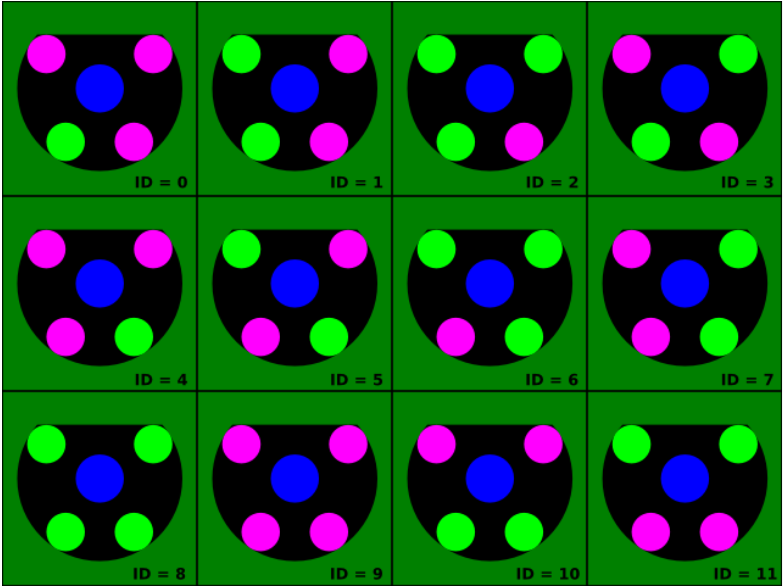
\includegraphics[width=0.8\linewidth]{padroes_ssl}
  \caption{Padrões oficiais da SSL~\cite{zickler-ssl}}\label{fig:padroes_ssl}
\end{figure}

A posição dos círculos que compõem o padrão são utilizados para calcular a orientação
e posiçao do robô no campo, conforme ilustrado na Figura~\ref{fig:rob_data}. Isso
tudo é feito pelo \textit{software} da SSL-Vision, que se utiliza das images capturadas
pelas duas câmeras posicionadas acima do campo. Esses dados são fornecidos em média a
cada $16,6{\ }ms$. A Figura~\ref{fig:cmra_campo} mostra a disposição das câmeras no
campo.

\begin{figure}[thpb]
  \centering
  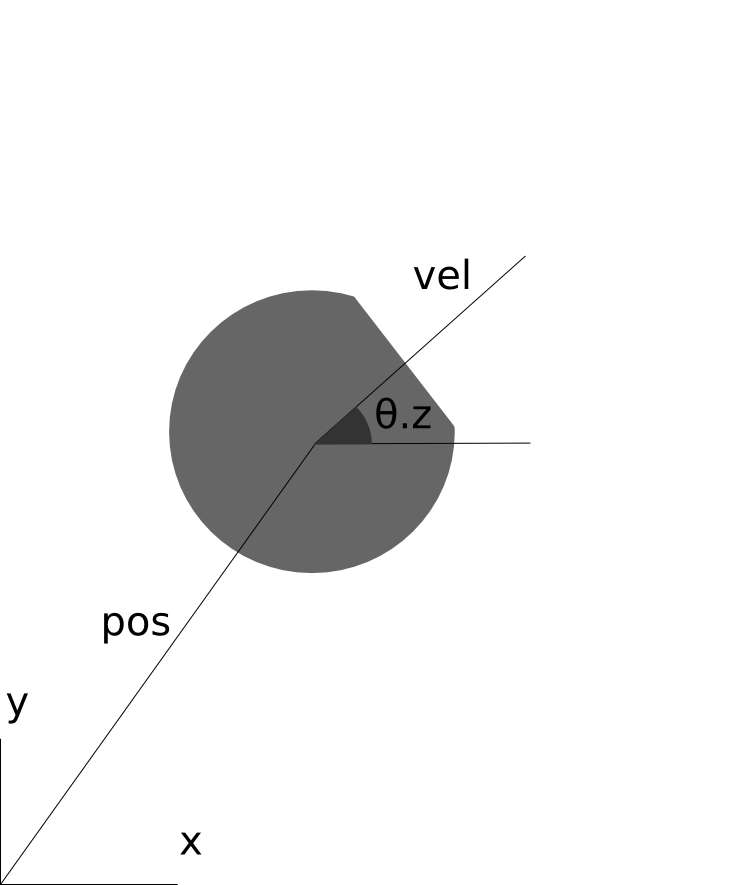
\includegraphics[width=0.5\linewidth]{img/rob_data}
  \caption{Parâmetros de estádo mutáveis do robô}\label{fig:rob_data}
\end{figure}

\begin{figure}[thpb]
  \centering
  \includegraphics[width= 0.8\linewidth]{img/cmra_campo}
  \caption{Disposição das câmeras no campo}\label{fig:cmra_campo}
\end{figure}

\begin{figure}[thpb]
  \centering
  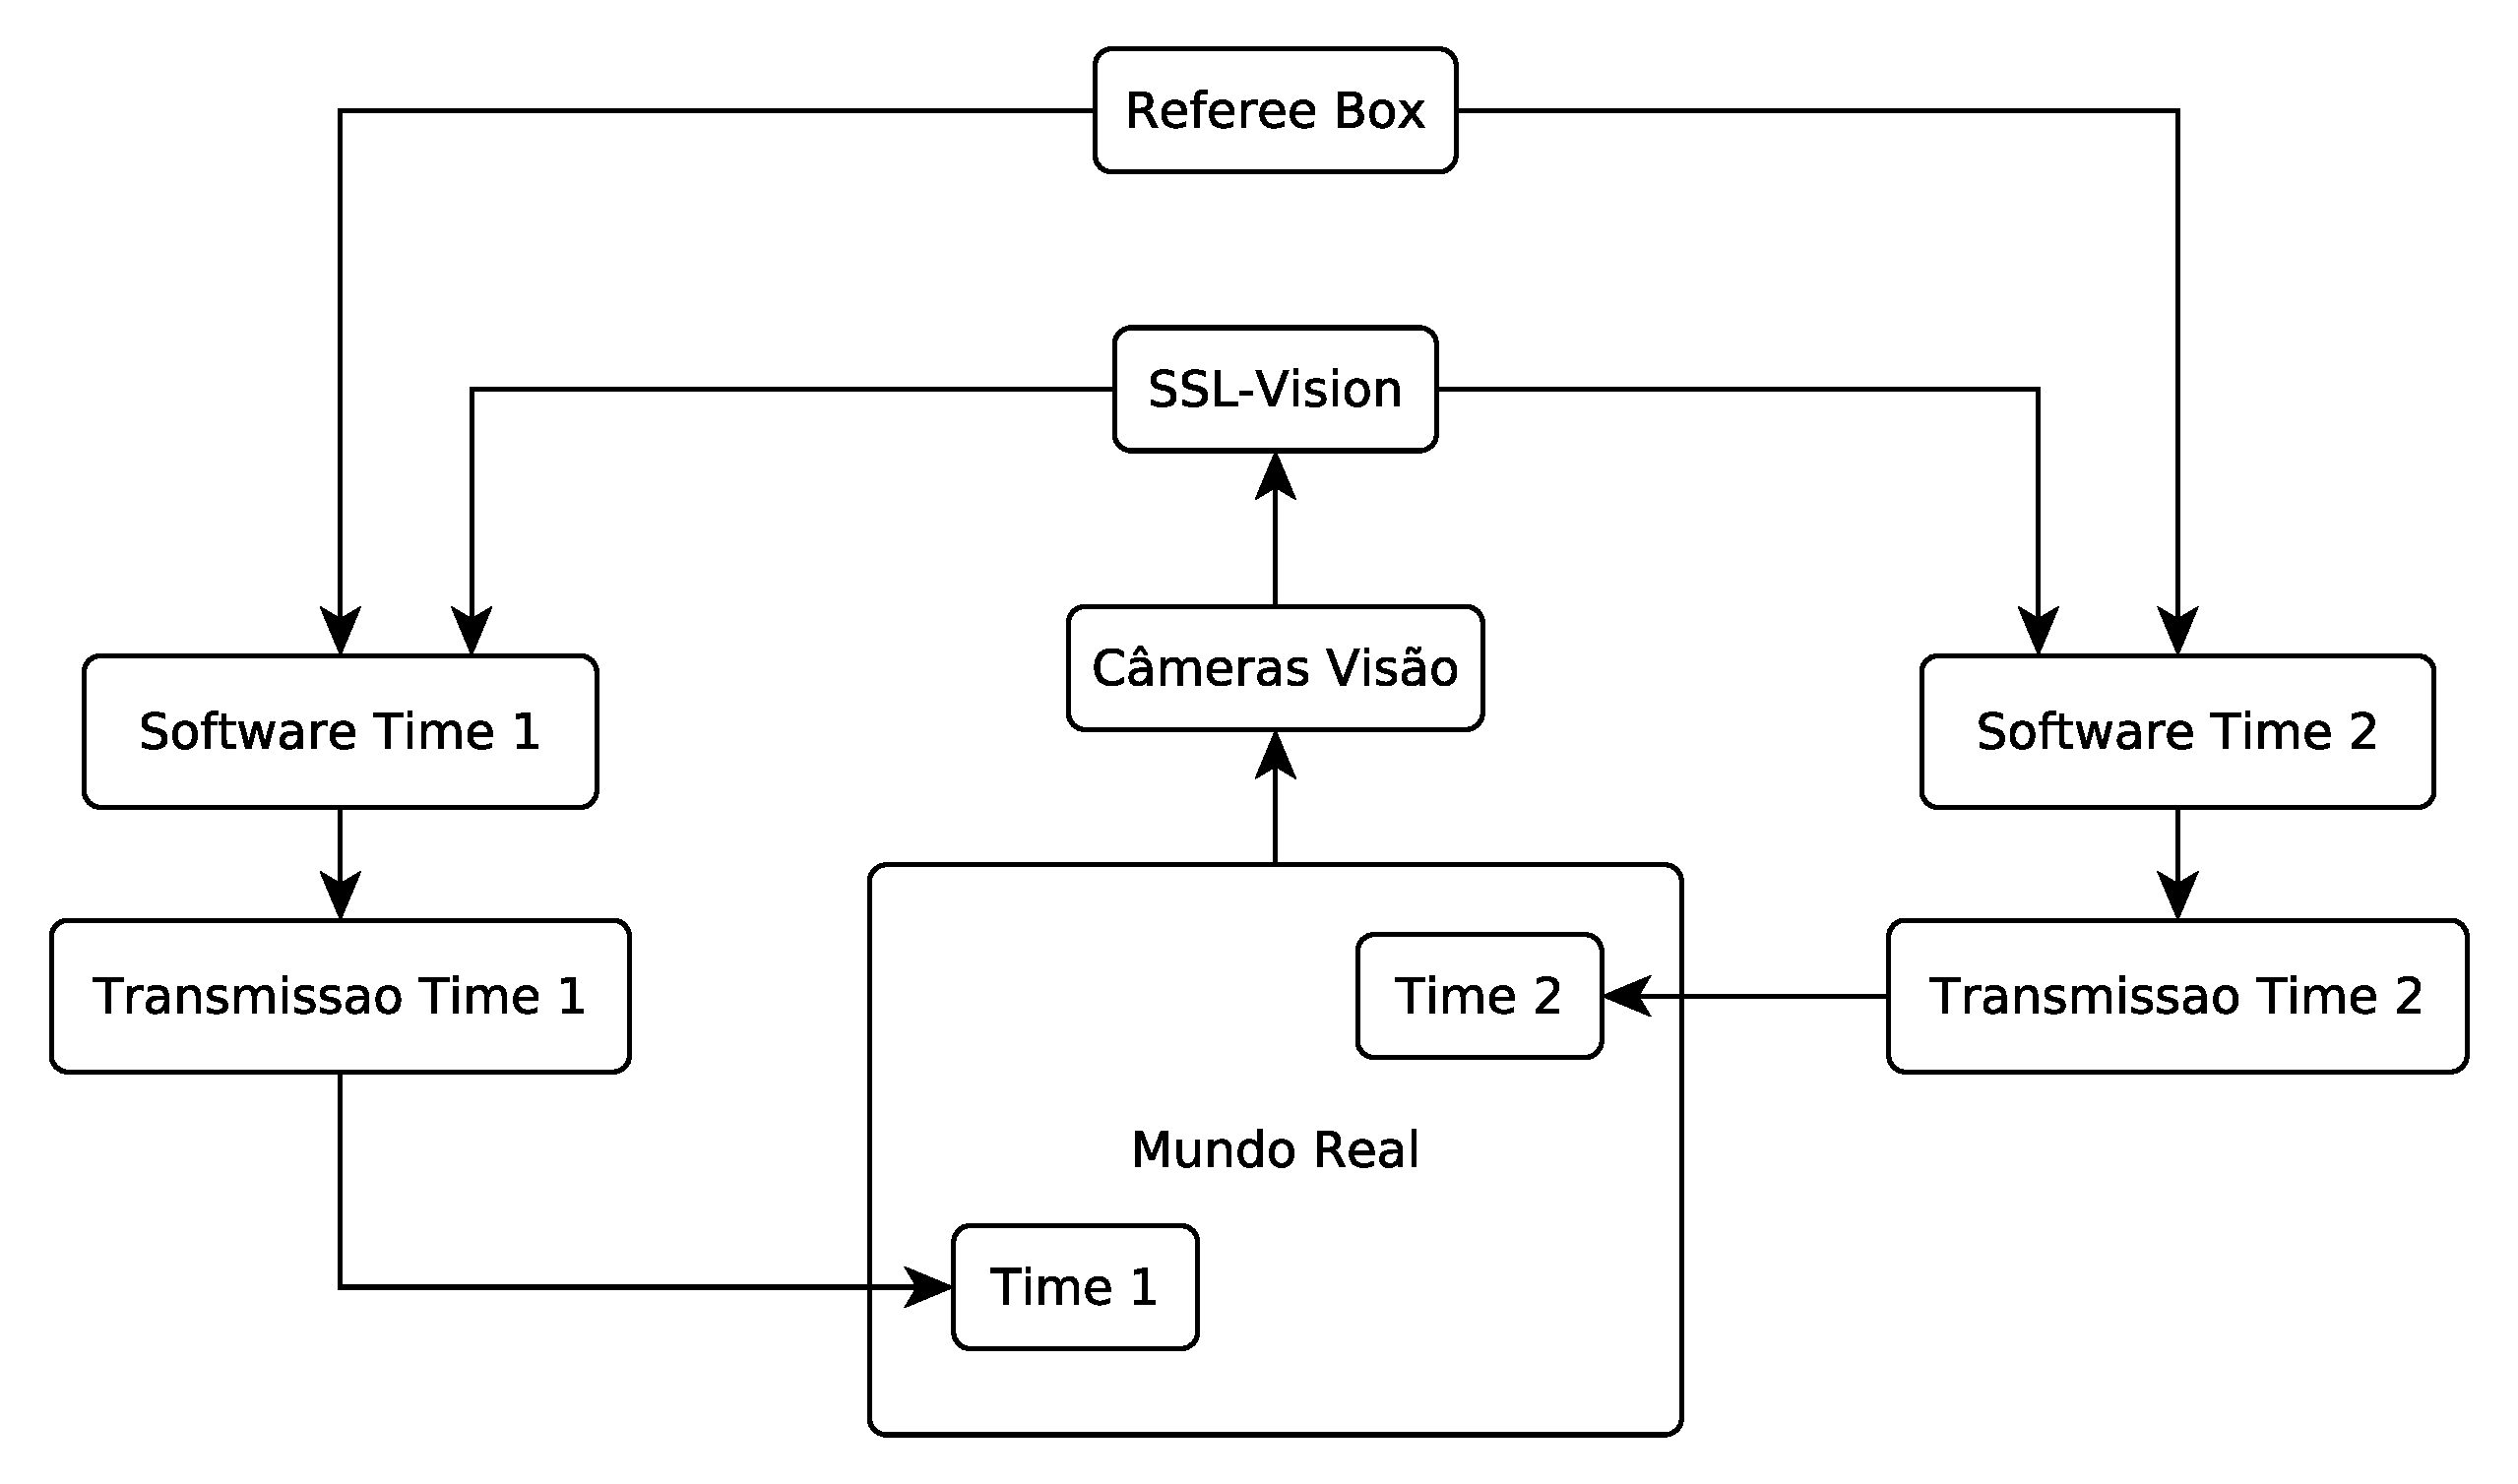
\includegraphics[width= 0.8\linewidth]{img/arq_ssl}
  \caption{Arquitetura básica da SSL}\label{fig:arquitetura_ssl}
\end{figure}

% vim: tw=80 et ts=2 sw=2 sts=2 ft=tex
